Po Janie przyszła na świat Stanisława, która urodziła się 22 I 1902 r. jak całe jej rodzeństwo w Mirowie. 

\begin{figure}[!h]
\begin{center}
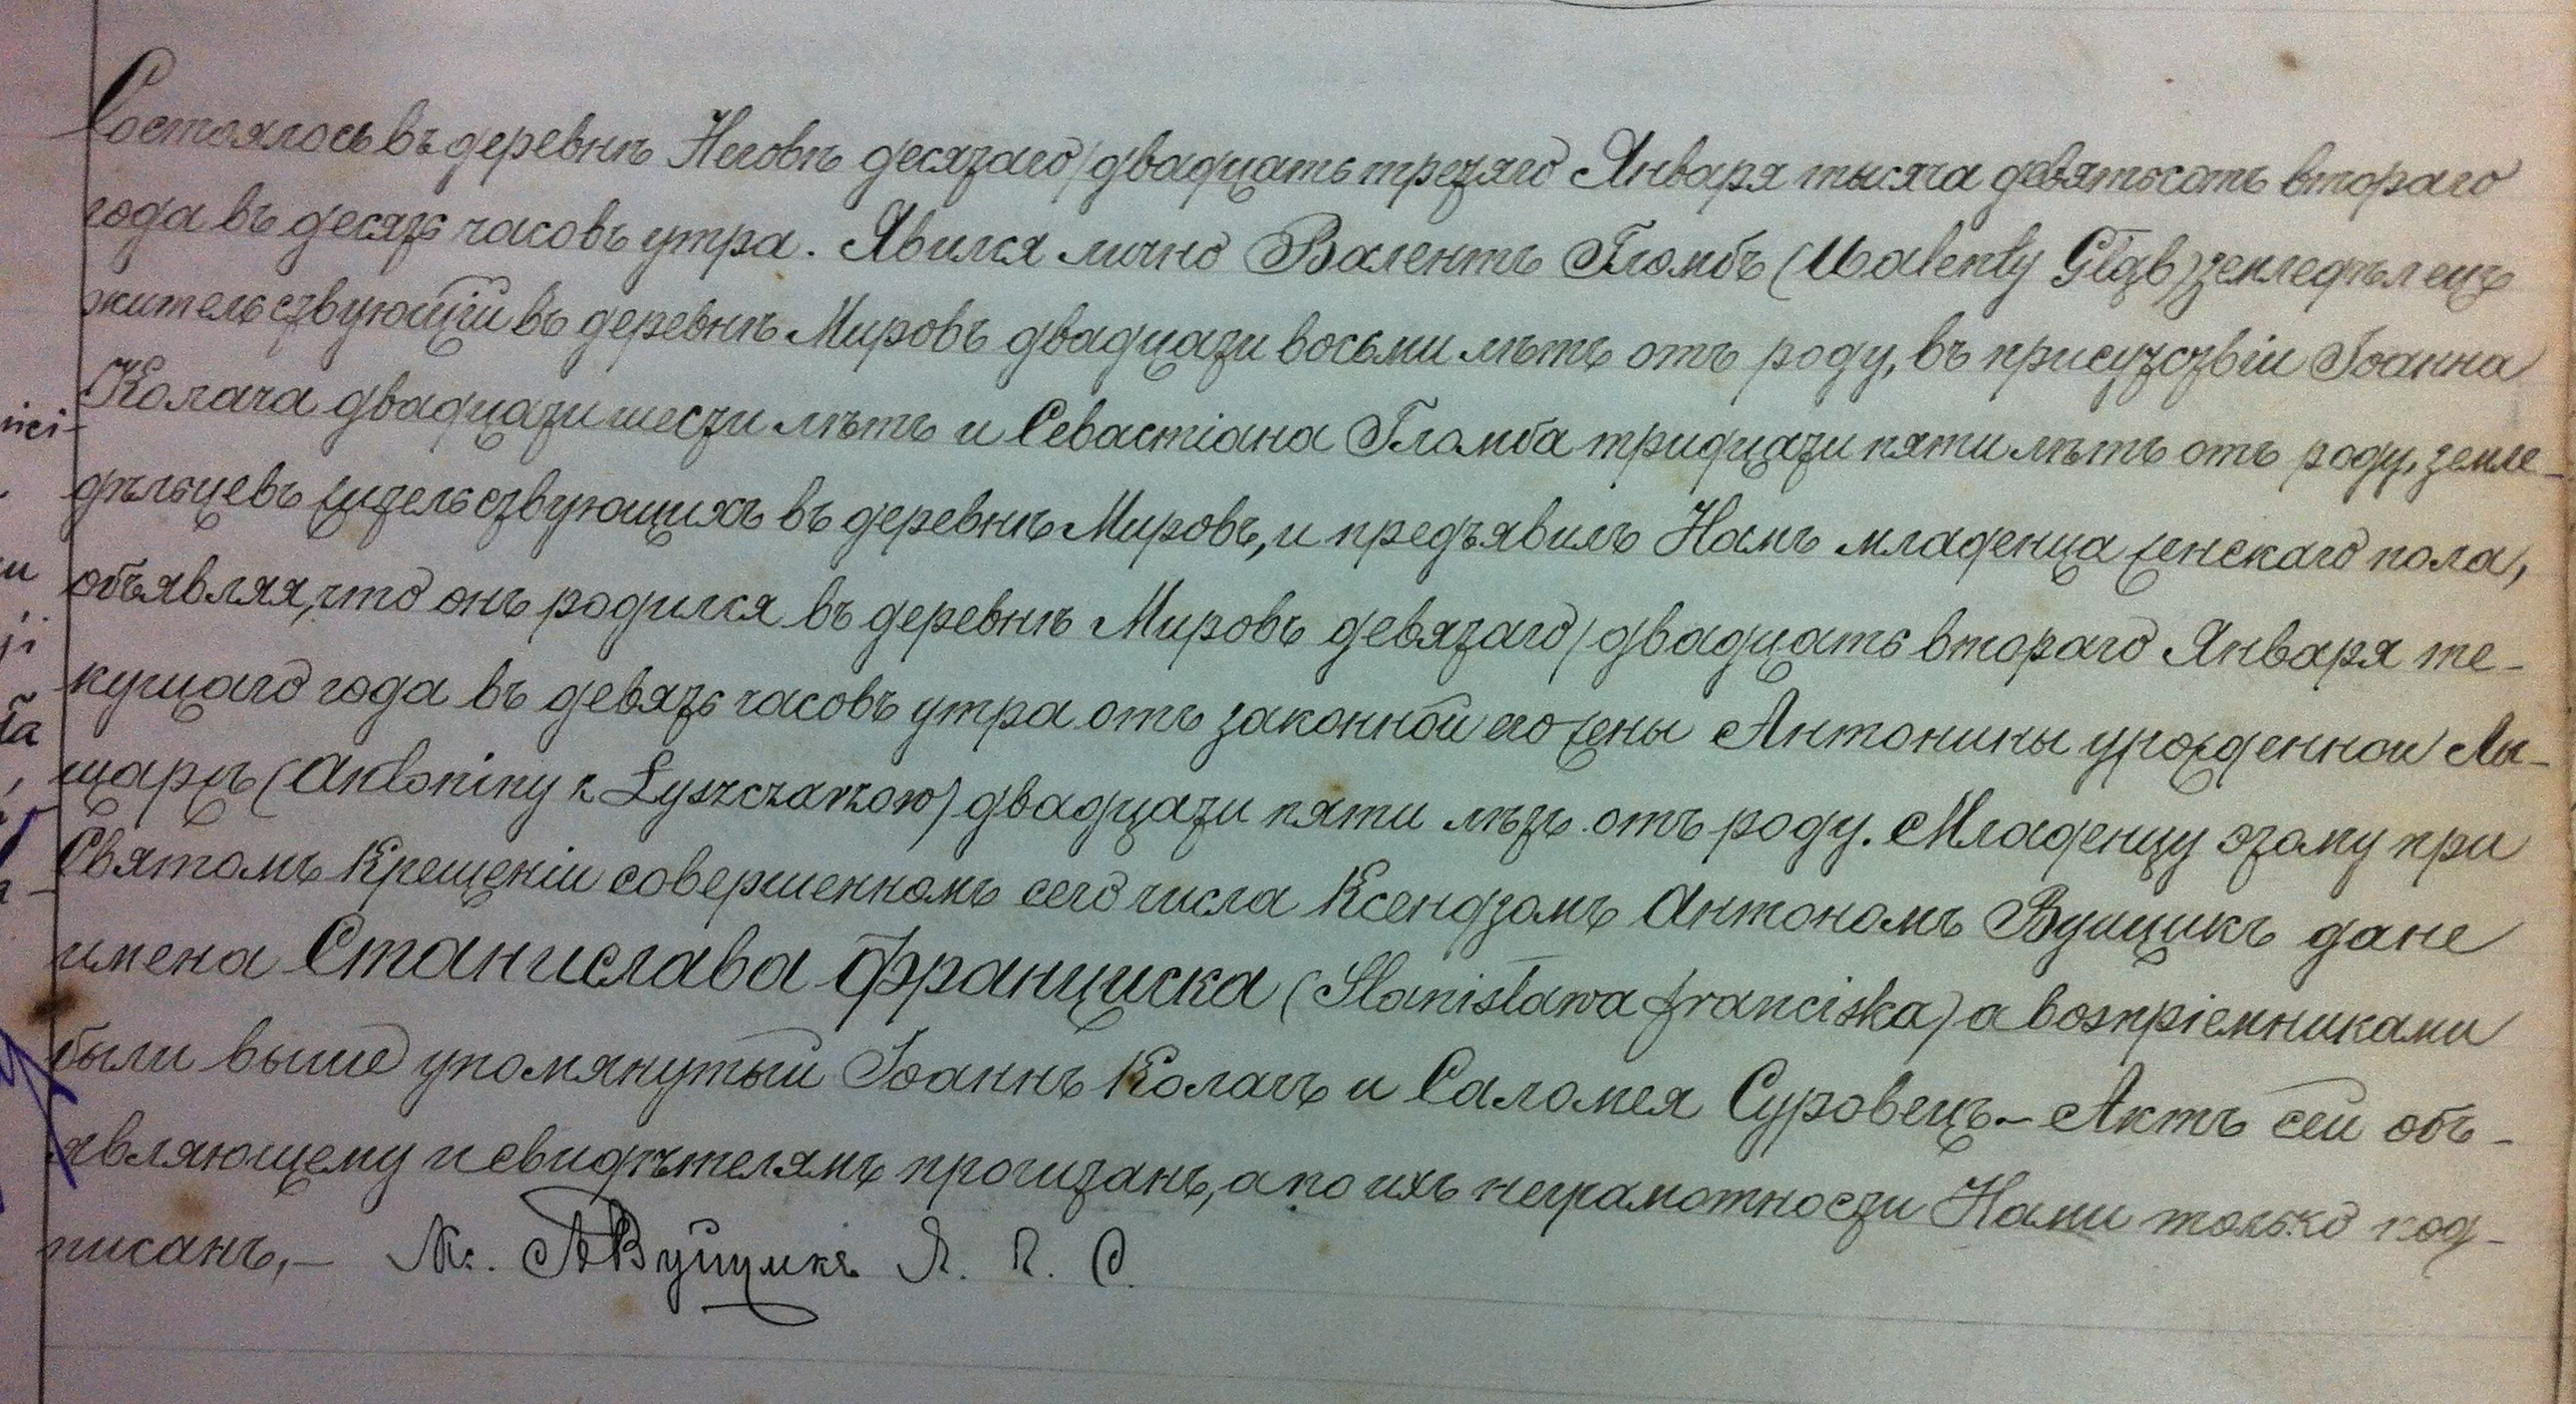
\includegraphics[width=0.8\textwidth]{zdjecia/akt_urodzenia_stanislawy_glab.jpg}
\caption[Akt urodzenia Stanisławy Głąb]{Akt urodzenia Stanisławy Głąb, córki Walentego i Antoniny z domu Łyszczarz}
\label{rys:akt_urodzenia_stanislawy_glab}
\end{center}
\end{figure}

Sama Stasia Głąbówna, jak pewnie całe rodzeństwo, nie miała łatwego życia u swoich rodziców. Gdy jako sześcioletnie dziecko musiała, na polecenie swego taty -- Walentego -- sprzątnąć łubin z pola, a ponieważ nie dała rady w porę tego zrobić, więc ją tatuś śmigał batem raz, drugi po gołych nogach, aż w końcu z wielkim płaczem ten łubin z pola sprzątnęła. Twarde było życie dzieci na wsi!

\begin{figure}[!ht]
\begin{center}
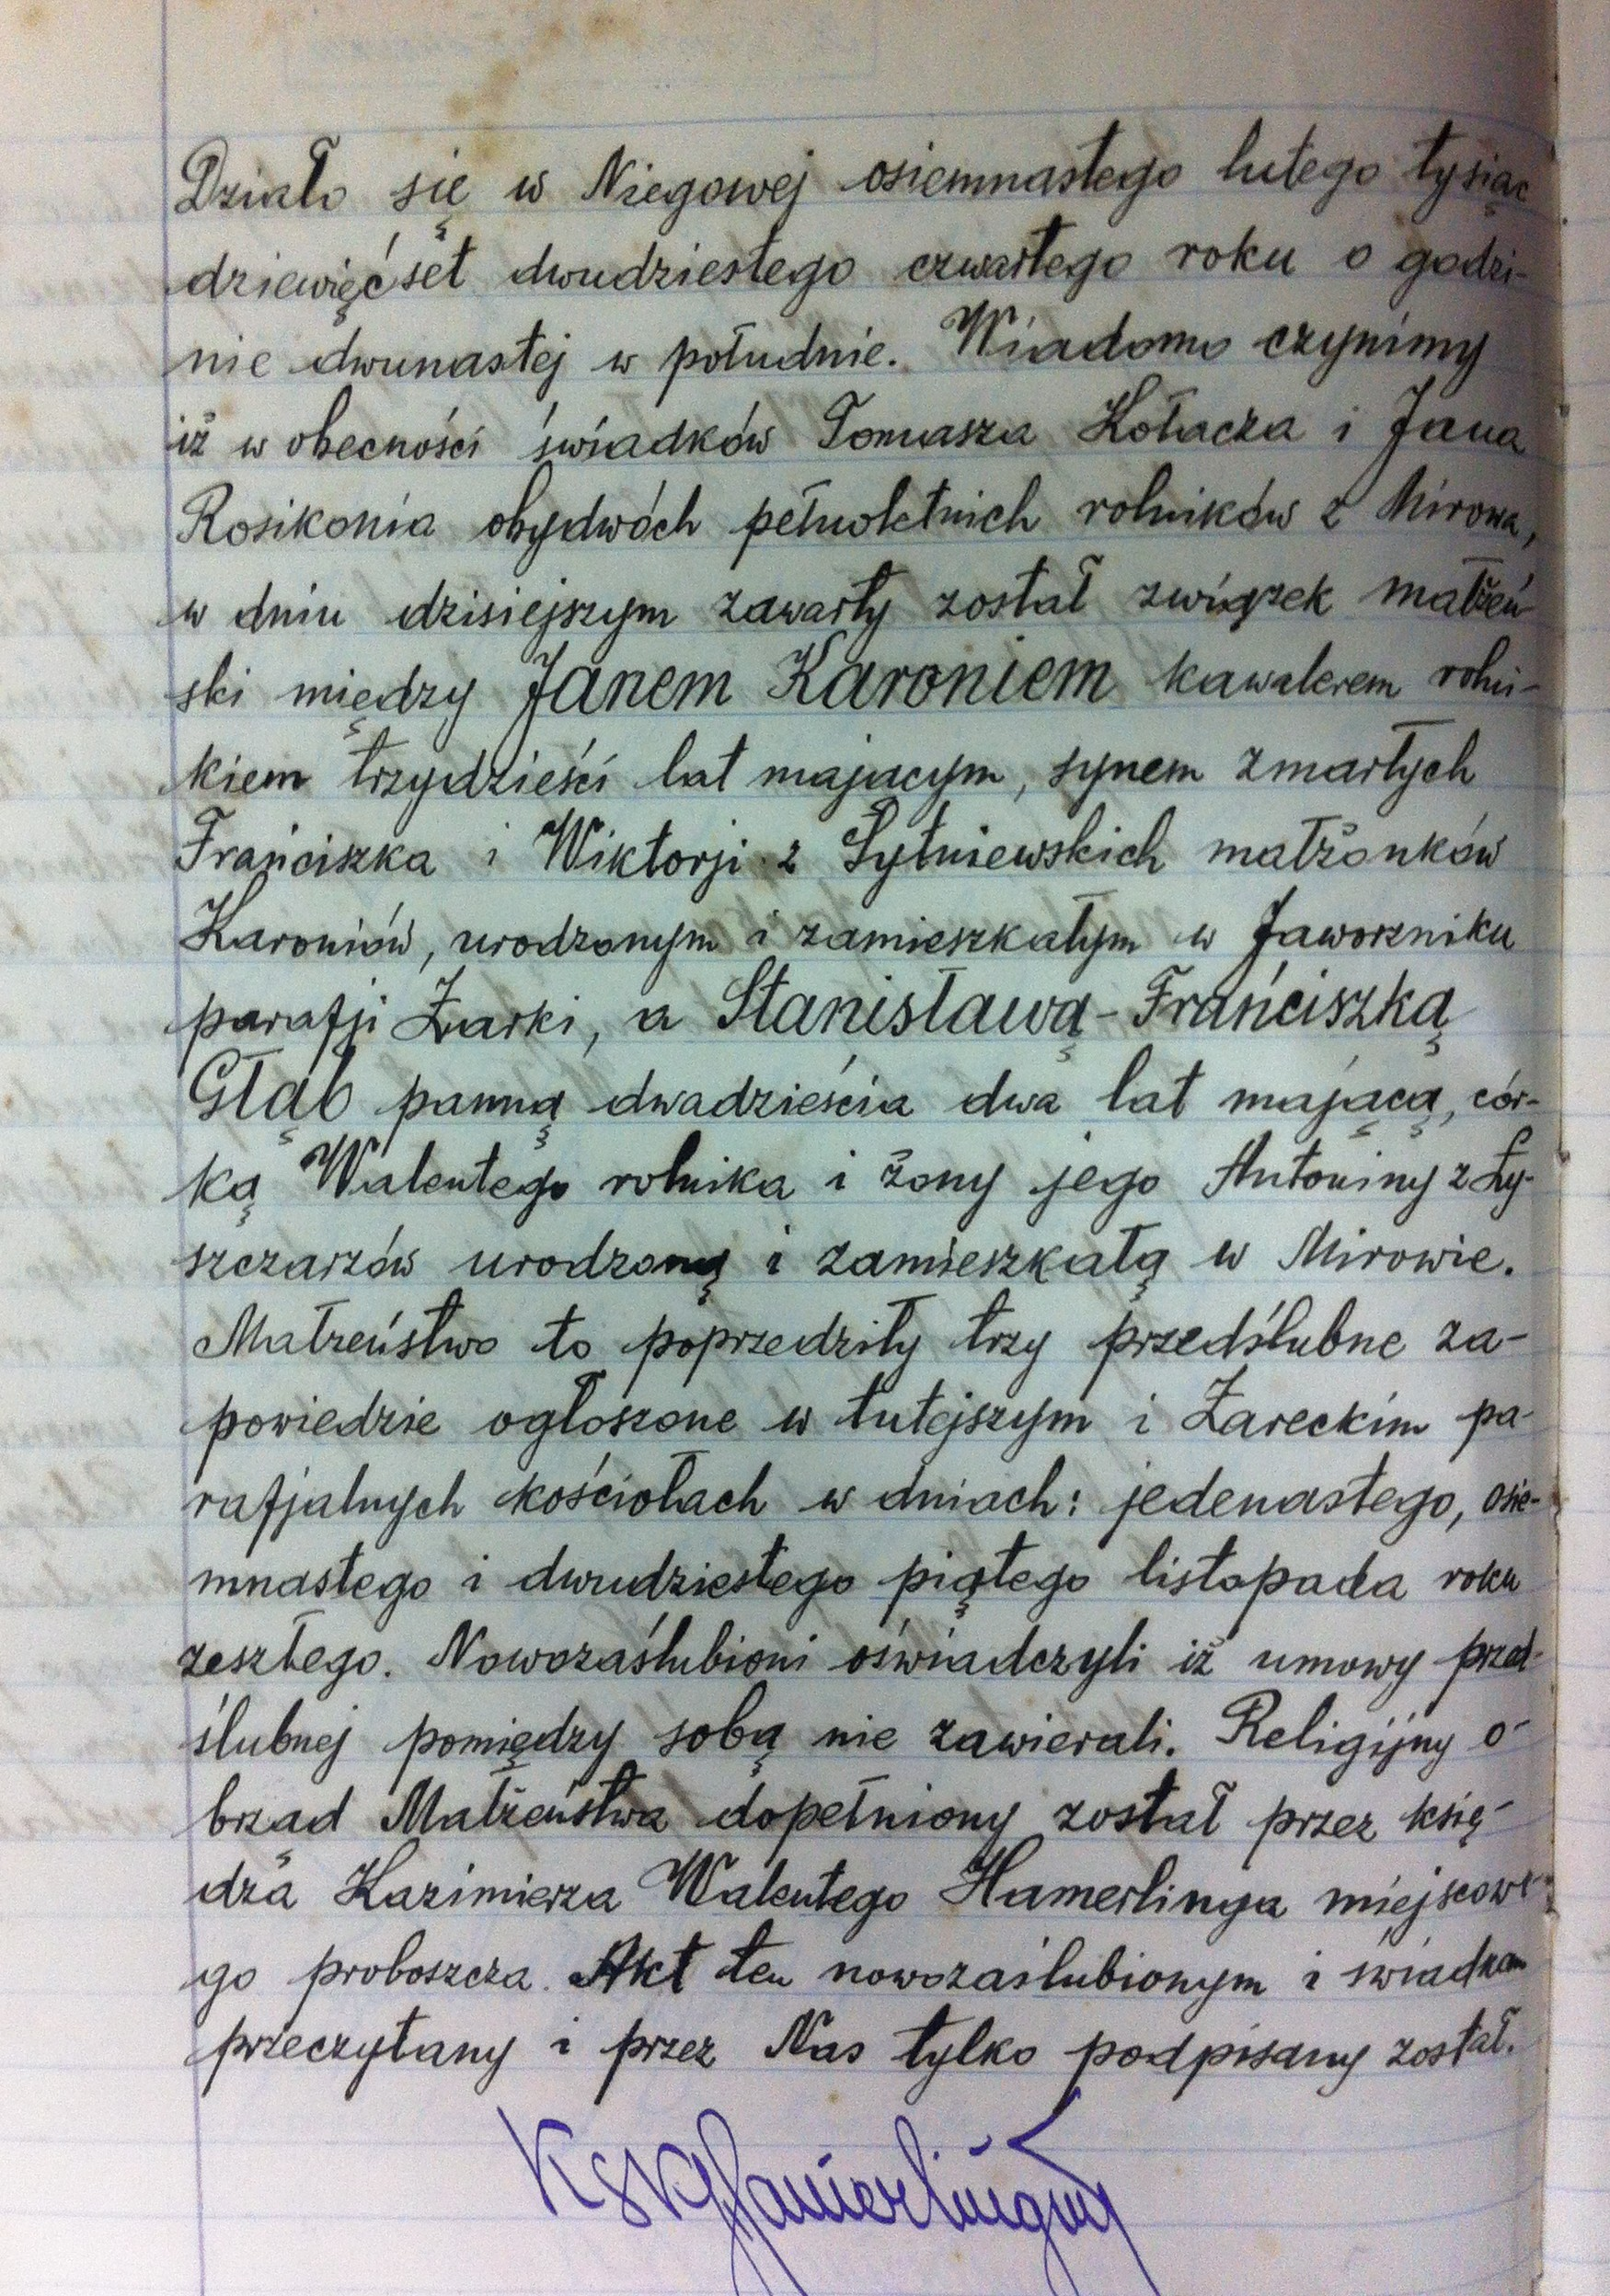
\includegraphics[width=0.52\textwidth]{zdjecia/akt_slubu_stanislawy_i_jana_karoniow.jpg}
\caption{Akt ślubu Stanisławy Głąb i Jana Karonia}
\label{rys:akt_slubu_stanislawy_i_jana_karoniow}
\end{center}
\end{figure}

\begin{figure}[!h]
\begin{center}
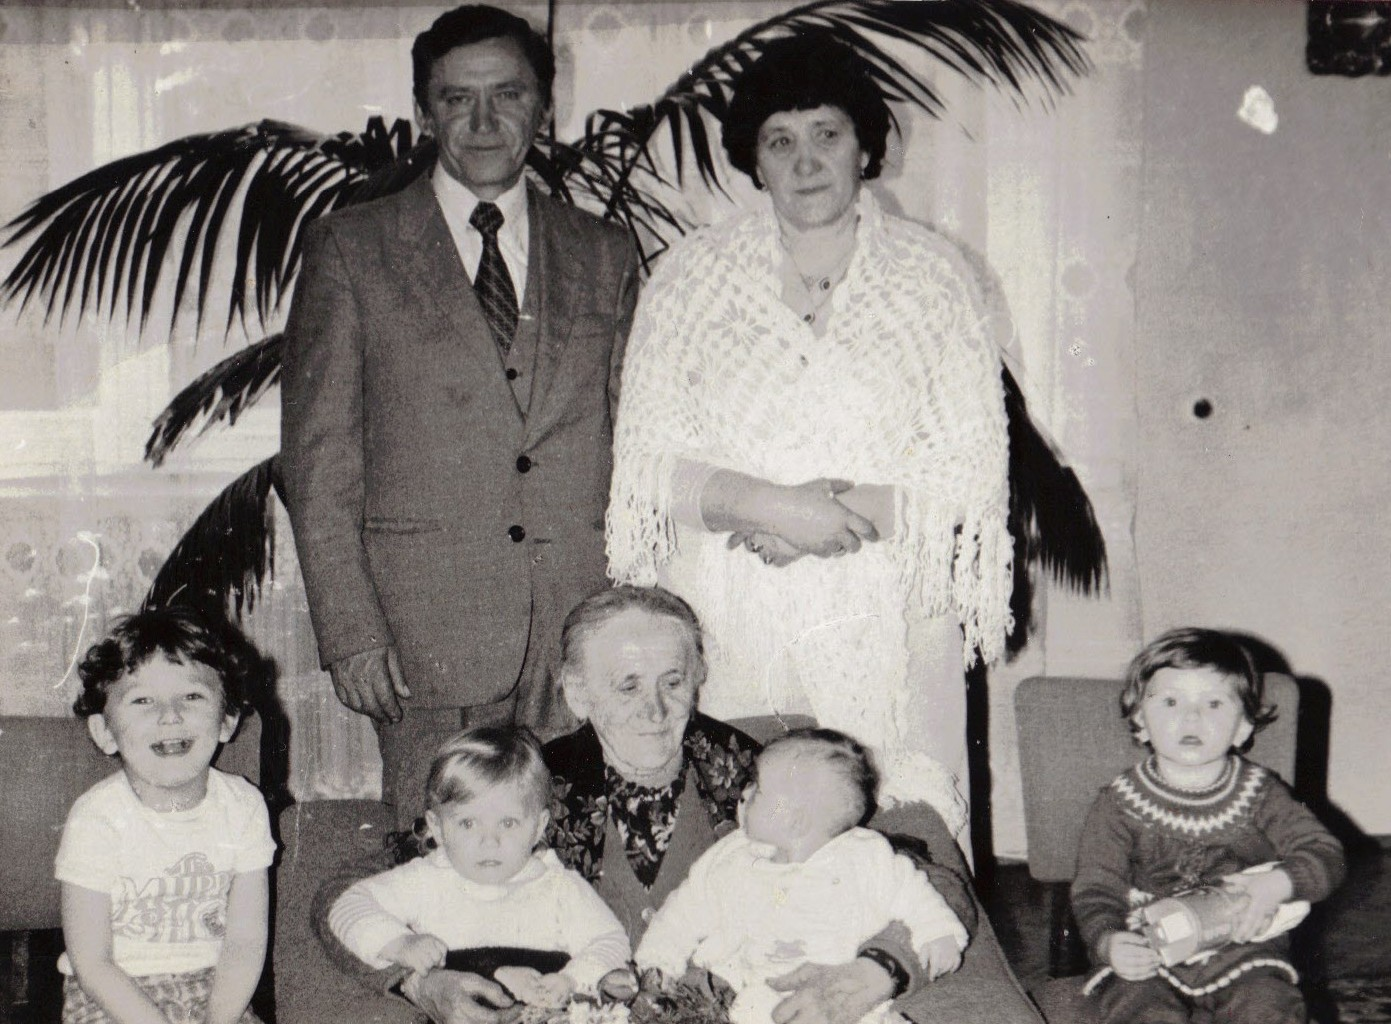
\includegraphics[width=0.7\textwidth]{zdjecia/statnislawa_karon_1.jpg}
\caption[Stanisława Karoń z rodziną]{Stanisława Karoń z domu Głąb siedząca z prawnukami, za nią stoją: córka Eleonora Bubel i syn Stanisław Karoń}
\label{rys:statnislawa_karon_1}
\end{center}
\end{figure}

Wyszła 18 II 1924 r. w Niegowie za Jana Karonia (ur. 6 XII 1893 r. w Jaworzniku z ojca Franciszka i Wiktorii z Sytniowskich).

Charakteryzowało się ich poprzez porównanie do ptaków, jako że Jan miał serce gołębia, a Stanisława serce jastrzębia. Była ona bowiem twarda nie tylko wobec innych, nawet swoich dzieci, lecz także wobec siebie. Gdy zbliżał się czas jej przejścia do wieczności, nie rozczulała się nad sobą, lecz mimo zaawansowanego wieku (85 lat) -- niezadowolona z wykonania remontu dachu stodoły, sama weszła na kalenicę, naprawiła, co tamci popsuli, lecz na koniec spadła stamtąd. W tym wieku taki wypadek zwykle kończył się śmiercią, a babka Stanisława naruszyła sobie piętę. Potem jeszcze tego roku miała obustronne zapalenie płuc i wyszła z tego!

Śmierć jednak nadal koło sędziwej Stanisławy krążyła, aż ją dopadła 5 grudnia 1987 r., gdy nieostrożnie wtargnęła na jezdnię w Jaworzniku koło przystanku autobusowego, przekonana, że to nadjeżdża autobus, na który nie mogła się spóźnić, bo miała być u swej córki Eleonory w Żarkach. Zmarł bowiem niedawno jej mąż -- Wacław Bubel, którego duch -- jej zdaniem -- buszował po ich domu, więc panicznie się bała sama spać u siebie. Spodziewany autobus okazał się samochodem osobowym, którego kierowca, skądinąd  bliski znajomy rodziny Karoniów, nie zamierzał przystawać na przystanku autobusowym. Stanisława Karoń wtargnęła na jezdnię z takim przeświadczeniem, że to autobus, iż nie dała kierowcy żadnych szans, wpadła prosto pod koła pojazdu i poniosła śmierć na miejscu.

Była też twarda dla swoich\ldots Gdy hitlerowcy przeprowadzali obławę na partyzantów w Jaworzniku, Stanisława kazała swemu czternastoletniemu synowi Stachowi zanieść meldunek do Góry Włodowskiej pod ostrzałem hitlerowców. Szczęściem, spotkał po drodze kogoś, kto mu powiedział, że adresat tego meldunku został właśnie przez Niemców zastrzelony.


\begin{figure}[!h]
\begin{center}
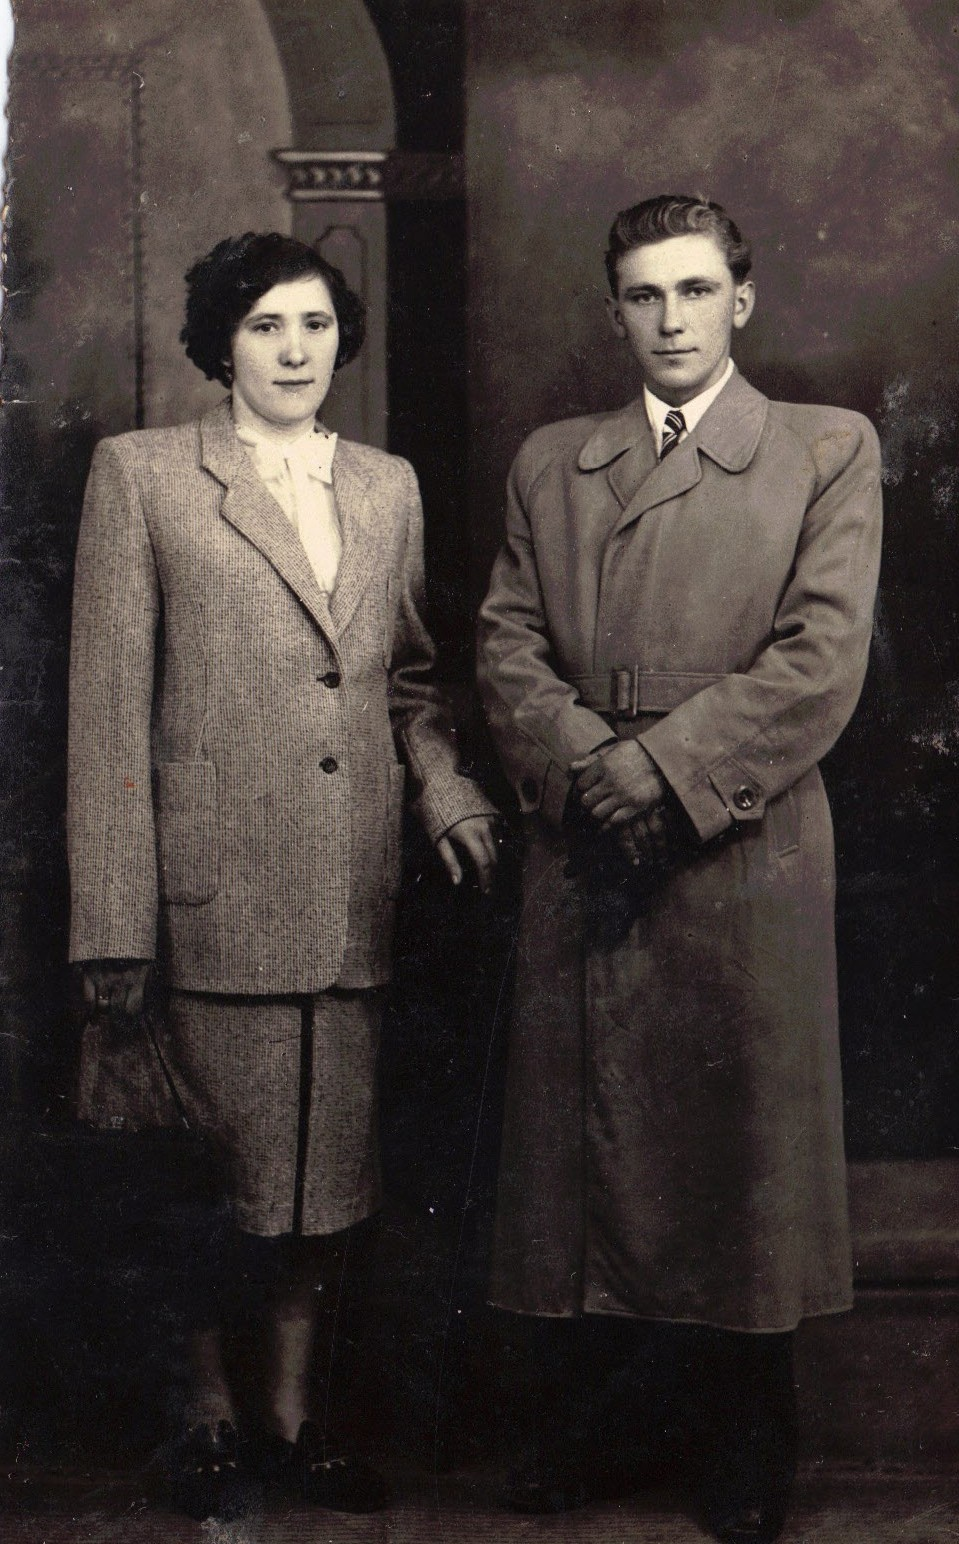
\includegraphics[width=0.4\textwidth]{zdjecia/eleonora_i_stanislaw_karoniowie.jpg}
\caption[Eleonora i Stanisław Karoniowie]{Eleonora i Stanisław Karoniowie - dzieci Stanisławy i Jana Karoniów}
\label{rys:eleonora_i_stanislaw_karoniowie}
\end{center}
\end{figure}

Stanisława Karoń bardzo dbała o to, by jej dzieci dobrze się prezentowały. Stachu Karoń na zdjęciu
%TODO - dodac odnosnik to zdjecia
dzieci z przedszkola jako jedyny ma muszkę. Szczególnie jednak dbała o prezencję swej córki -- Eleonory. Była ona na 40 weselach jako druhna i na każdym weselu była w innej sukni (więc miała 40 sukien), co było wielkim wydatkiem. Można było nie dojeść, nawet głodować, można było żyć w zimnie, ale na zewnątrz należało się pokazać! Stąd u Stanisławy Karoń taki szacunek dla pieniędzy\ldots Ktoś, kto miał pieniądze, był dla niej godnym szacunku. Stąd pierwszy kawaler Leosi Karoniówny -- Alfred Czyż -- jakiś wojskowy nie znalazł akceptacji w oczach matki, bo był biedny. Podobno za nim ciotka Leosia oczy wypłakała. Wyszła za syna sąsiadów z ,,Górki'' -- Wacława Bubla, który był majętny i na tyle cwany, że swą wybrankę uczynił brzemienną jeszcze przed ślubem.

\begin{figure}[!h]
\begin{center}
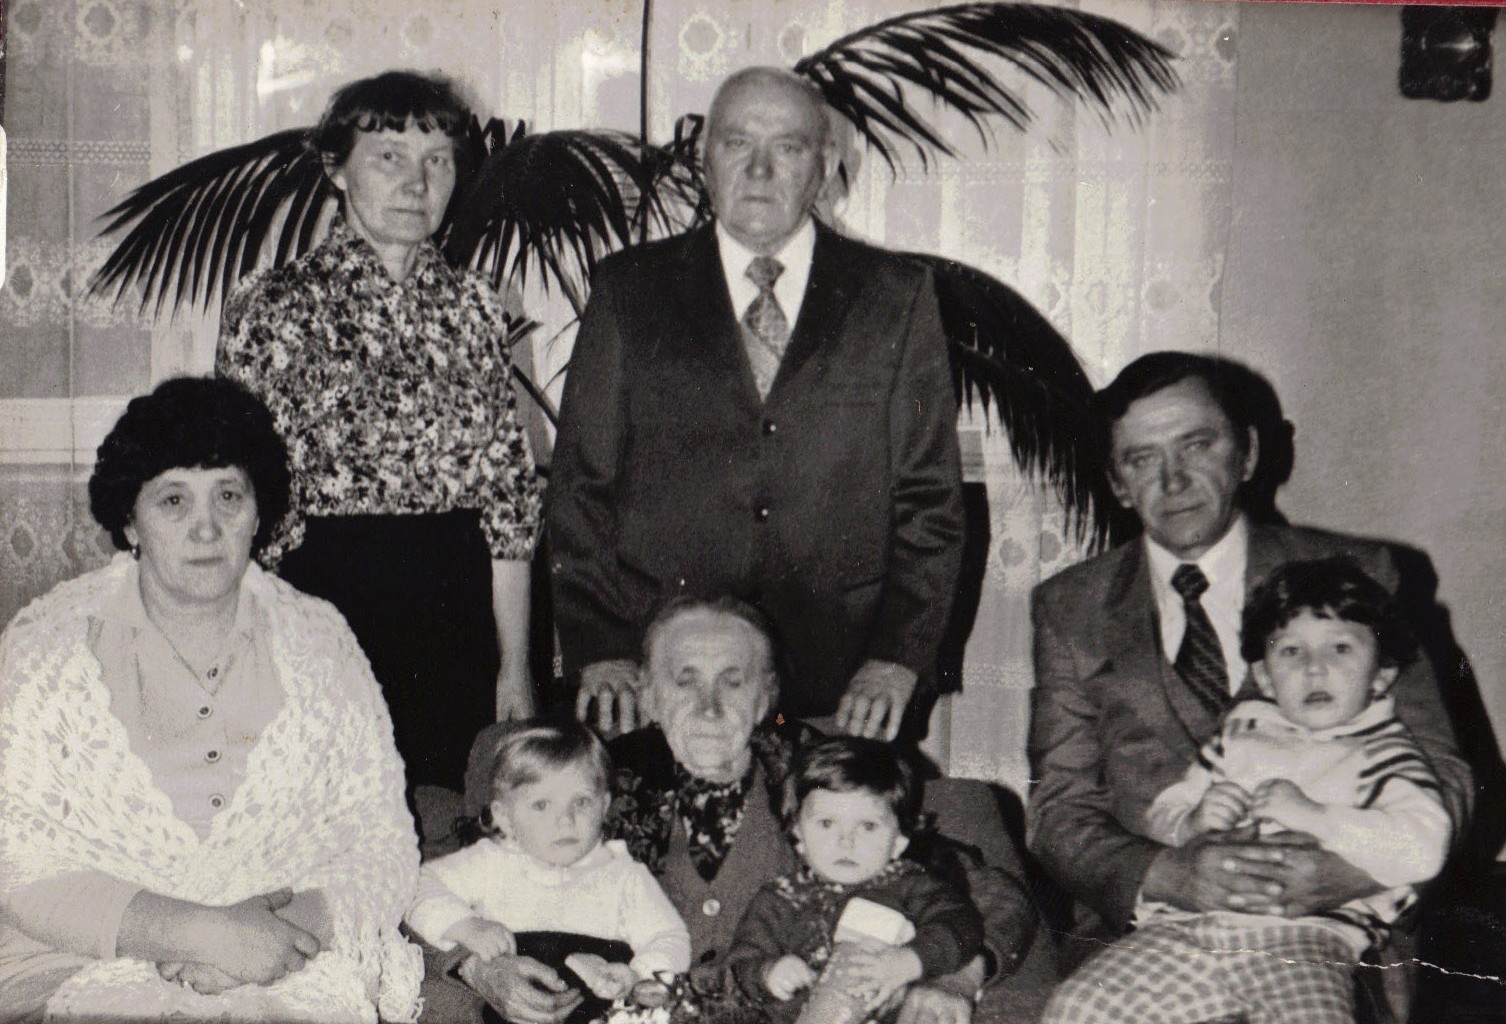
\includegraphics[width=0.75\textwidth]{zdjecia/eleonora_i_waclaw_bublowie.jpg}
\caption[Eleonora i Wacław Bublowie]{Stoją: Zofia Karoń (żona Stanisława) i Wacław Bubel, siedzą od lewej: Eleonora Bubel (żona Wacława), jej matka, Stanisława z prawnuczkami i Stanisław Karoń z wnukiem Przemysławem Karoniem}
\label{rys:eleonora_i_waclaw_bublowie}
\end{center}
\end{figure}
Stanisław Karoń był bardzo zdolnym chłopcem, zwłaszcza w matematyce i dlatego nadawał się do technikum mechanicznego w Katowicach. Nawet rozpoczął tam naukę, ale matka Stanisława kategorycznie się sprzeciwiła, bo ,,trzeba robić pieniądze'' i tak Stachu został z podstawówką, ale pieniądze zawsze miał. Szkoda tylko człowieka! Kto wie kim byłby ów zdolny chłopiec, gdyby wyjrzał na świat przez okna tego technikum?! A potem może byłyby studia? Ojciec Jan, jak to gołąb przy jastrzębiu, nie miał wiele do powiedzenia\ldots Stanisława Karoń była bardzo aktywna, najruchliwsza z całego rodzeństwa. Ta jej nadzwyczajna żywotność nie wszędzie i nie zawsze była mile widziana. Kojarzeniem par zajmowała się prawie do końca życia.

Natomiast Jan Karoń również bardzo aktywny, ale zawsze w trosce o ciepło rodzinne, by dzieciom było dobrze i by dobrze mogli o nim mówić ci, co z nim wchodzili w jakieś stosunki. Uczciwy w transakcjach handlowych, danemu słowu był zawsze wierny. Doczekali się oni trójki dzieci, z tego dwoje dożyło wieku dojrzałego: córka Eleonora ur. 14 I 1925 r. w Jaworzniku oraz Stanisław Karoń ur. 22 VII 1928 r. również w Jaworzniku.

Jan Karoń zmarł 7 X 1970 r. w Jaworzniku, a jego małżonka Stanisława z domu Głąb siedemnaście lat później 5 XII 1987 r. w Jaworzniku.


\section{Eleonora Bubel}

Eleonora wyszła za Wacława Bubla (ur. 8 VIII 1912 r. w Jaworzniku, zm. 29 XI 1987 r.) i miała z nim trójkę dzieci: syna Longina (ur. 25 VIII 1947 r. w Żarkach, zmarł 20 XI 2006 r. w Żarkach w stanie kawalerskim), młodszego odeń o trzy lata Leszka (ur. 20 II 1950 r. w Żarkach) oraz najmłodszą Małgosię (ur. 4 IX 1955 r. w Żarkach). Lońka widzimy na zdjęciu ślubnym Mariana i Mieci Szczepańczyków (rys.~\ref{rys:slub_mieczyslawy_i_mariana_szczepanczykow}).

\begin{figure}[!h]
\begin{center}
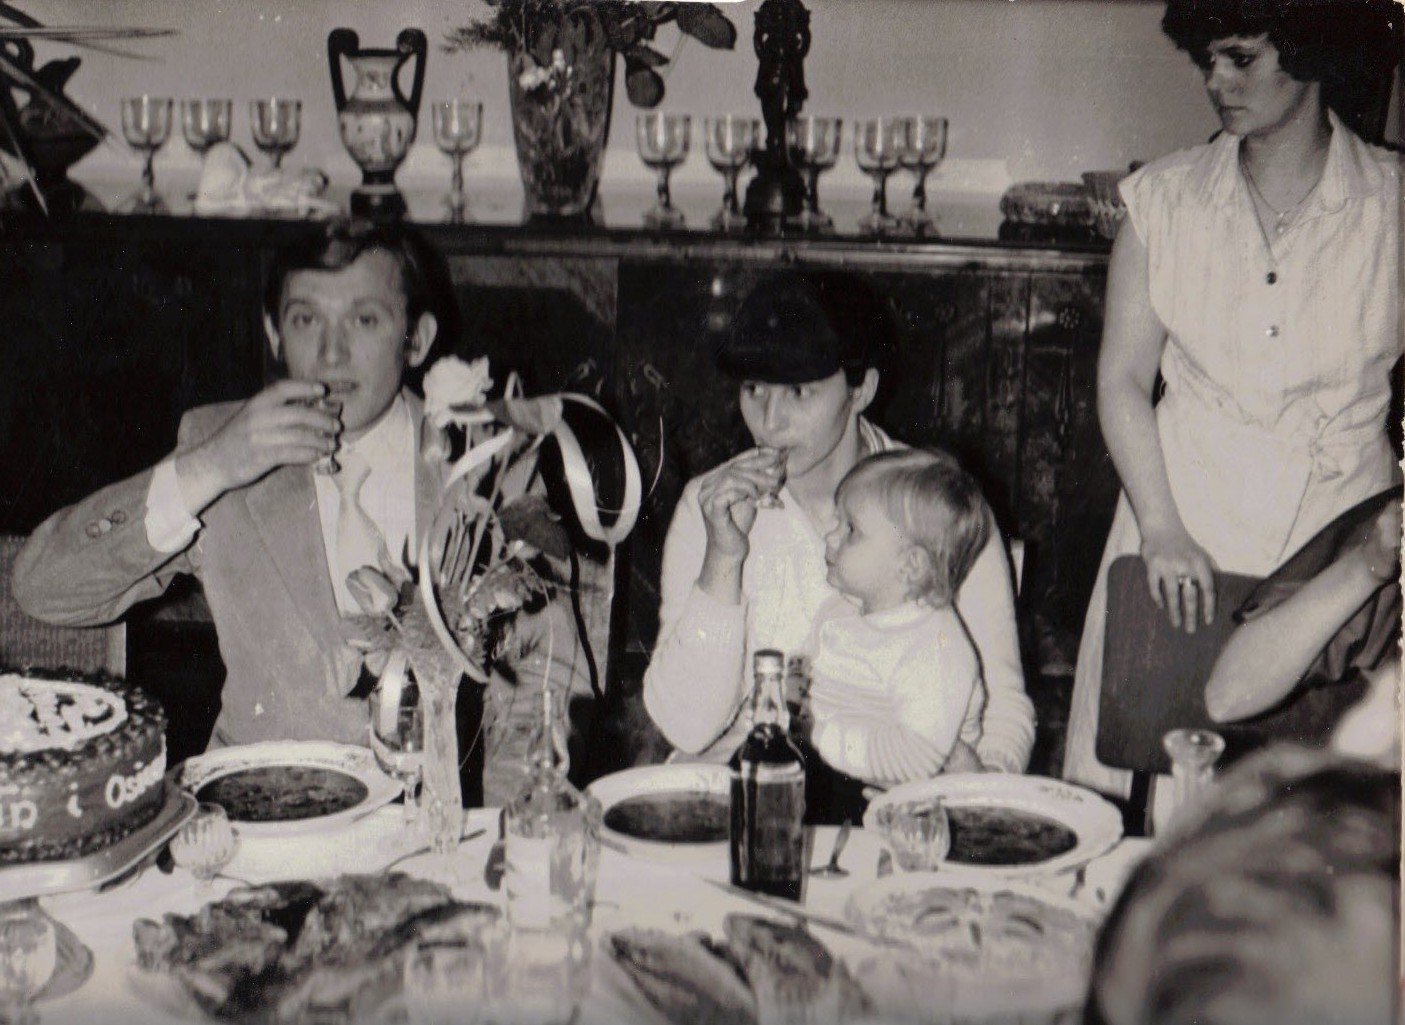
\includegraphics[width=0.7\textwidth]{zdjecia/leon_henryka_malgosia_bubel.jpg}
\caption[Leon, Henryka i Małgorzata Bublowie]{Na zdjęciu od lewej: Leon (Leszek) Bubel, jego żona Henryka z domu Kołodziejczyk z dzieckiem, stoi siostra Leszka -- Małgosia Mazur z domu Bubel}
\label{rys:leon_henryka_malgosia_bubel}
\end{center}
\end{figure}

Leon Bubel zwany Leszkiem ożenił się 17 IV 1976 r. w Żarkach z uroczą Henią Kołodziejczykówną z Jaworznika (ur. 14 IV 1956 r. w Żarkach z ojca Andrzeja i matki Władysławy z domu Kot). Ma z nią trójkę już dorosłych dzieci: córkę Renatę (ur. 10 VIII 1975 r. w Myszkowie), syna Marcina (ur. 24 X 1976 r. w Myszkowie) oraz syna Artura (ur. 28 III 1981 r. w Żarkach). Renata Bublówna wyszła dnia 12 maja 2007 r.
za Marka Wiewiórę (ur. 17 VI 1978 r. z ojca Tadeusza i matki Zofii z Bańskich), ale nie doczekali się jeszcze potomstwa. Marcin Bubel jest nadal kawalerem. Najmłodszy Artur Bubel ożenił się 26 lipca 2008~r. z Joanną Morawiec (ur. 13 IV 1981 r. z ojca Krzysztofa i matki Ewy z Kurzyków) i ma z nią syna Damiana (ur. 24 IV 2010 r.).

\begin{figure}[!h]
\begin{center}
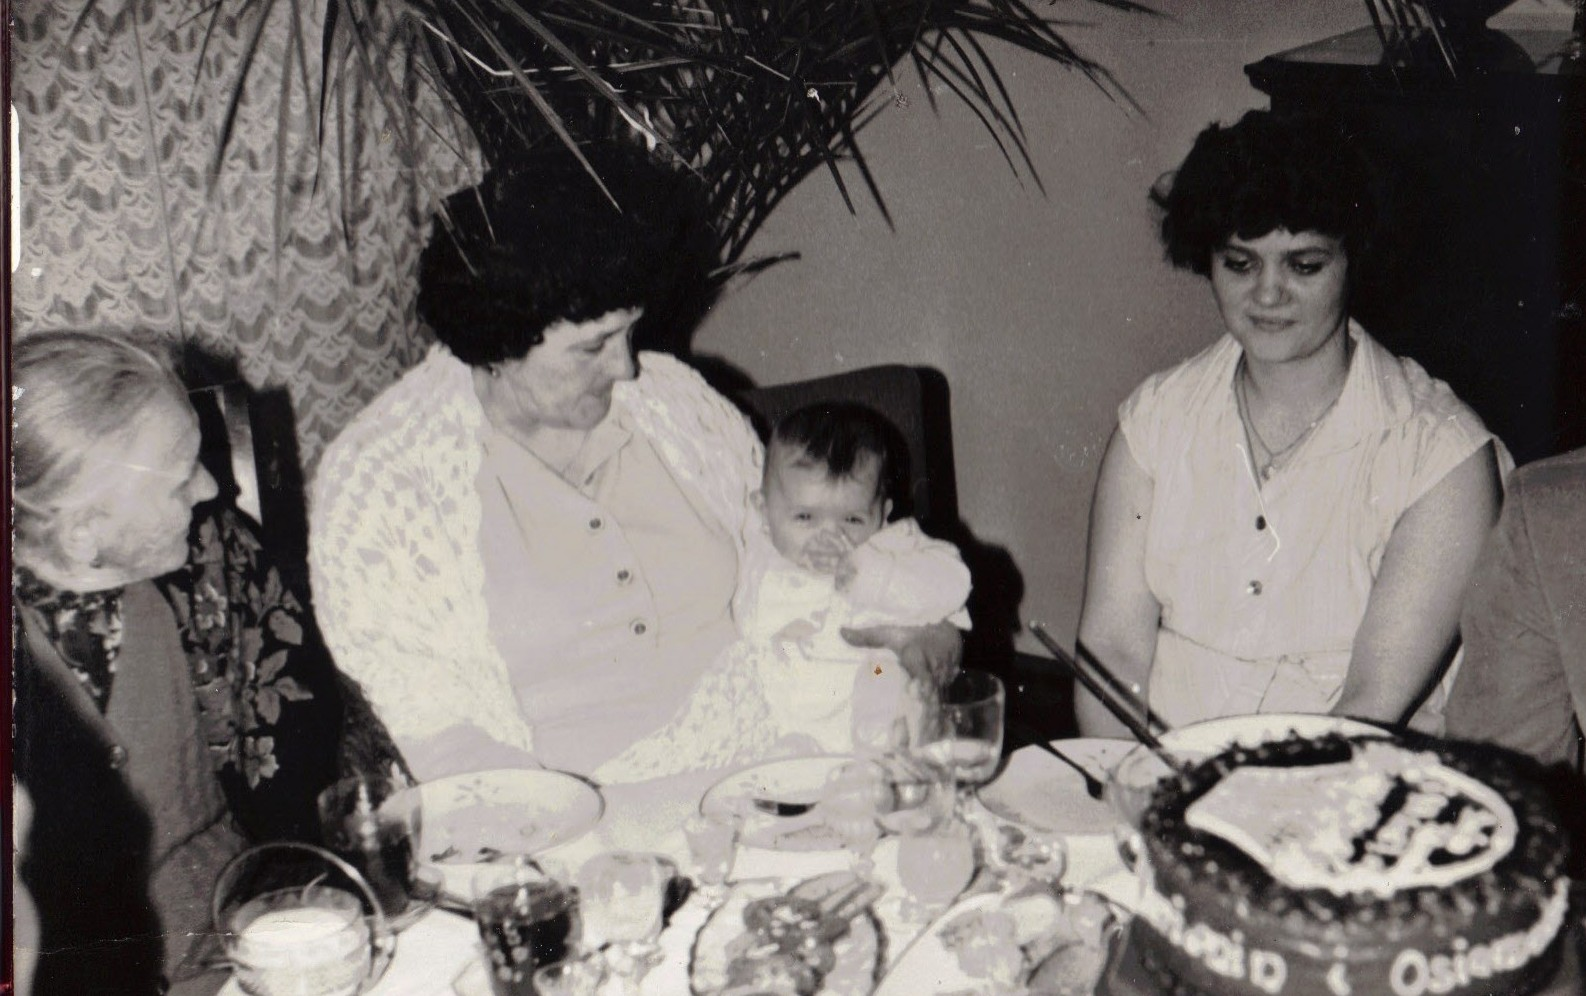
\includegraphics[width=0.6\textwidth]{zdjecia/stanislawa_karon_eleonora_i_malgorzata_bublowie.jpg}
\caption[Osiemdziesiątka Stanisławy Karoń - cztery pokolenia]{Osiemdziesiątka Stanisławy Karoń z domu Głąb (po lewej). Od prawej Małgorzata Bubel, wnuczka, Eleonora Bubel, córka z prawnuczką jubilatki}
\label{rys:stanislawa_karon_eleonora_i_malgorzata_bublowie}
\end{center}
\end{figure}

Małgosia Bublówna wyszła 28 lutego 1981 r. za Andrzeja Mazura (ur. 29 V 1952 r. w Jędrzejowie z ojca Jana i matki Haliny z Urbanów) i ma z nim troje dorosłych już dzieci: córkę Annę (ur. 10 XI 1981 r. w Kędzierzynie), syna Michała (ur. 24 VII 1985 r. w Kędzierzynie) oraz syna Bartosza (ur. 27 IX 1989 r. w Kędzierzynie). Do tej pory związek małżeński zawarła córka Anna z Adamem Buzo.

\section{Stanisław Karoń}

\begin{figure}[!b]
\begin{center}
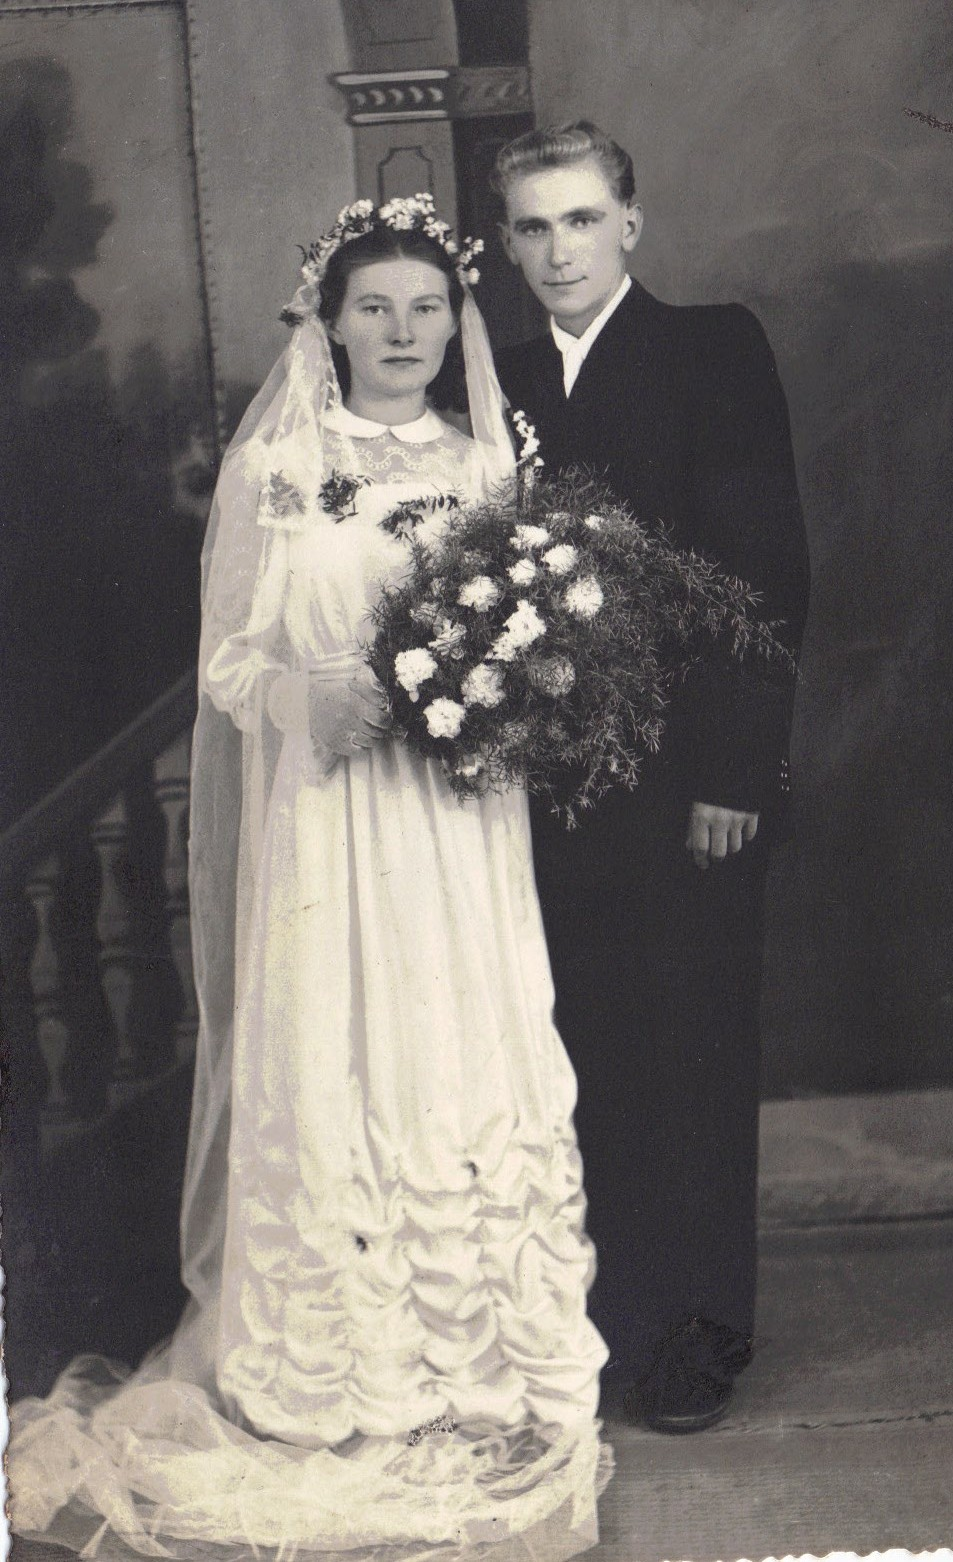
\includegraphics[width=0.4\textwidth]{zdjecia/slub_stanislawa_i_zofii_karon.jpg}
\caption{Zdjęcie ślubne Zofii Czyżówny ze Stanisławem Karoniem}
\label{rys:slub_stanislawa_i_zofii_karon}
\end{center}
\end{figure}

Stanisław Karoń ożenił się 3 VIII 1953 r. w Żarkach z Zosią Czyżówną (ur. 7 XII 1931 r. w Jaworzniku), z którą ma dwóch synów: Krzysztofa Karonia (ur. 27 V 1954 r. w Leśniowie) oraz Jarosława Karonia (ur. 8 VIII 1955 r. w Żarkach). Jednak pierwszy ożenił się Jarosław dnia 9 IX 1979 r. w Złotym Potoku z Marią Serafin ur. 1 V 1952 r. w Głuchołazach. Ma z nią dwoje dzieci: syna Przemysława (ur. dnia 10 XI 1978 r.) w Kędzierzynie Koźlu oraz córkę Annę (ur. dnia 8 IX 1980 r. w Kędzierzynie Koźlu). Przemek Karoń ożenił się 18 VIII 2005 r. w Ostrowcu Świętokrzyskim z Agnieszką Łatą (ur. 6 V 1978 r. w Skarżysku Kamiennej). Ma z nią dwie córki: Zosię Karoń ur. 14 V 2005 r. oraz Olę Karoń ur. 10 VI 2008 r. -- obie urodzone w Kędzierzynie Koźlu. Ania Karoń wyszła dnia 26 VIII 2007 r. w Kędzierzynie Koźlu za Tomasza Jamieluchę (ur. 10 IX 1982 r.), z którym ma córkę Hannę (ur. 17 III 2010 r. w Kędzierzynie Koźlu).

\begin{figure}[!h]
\begin{center}
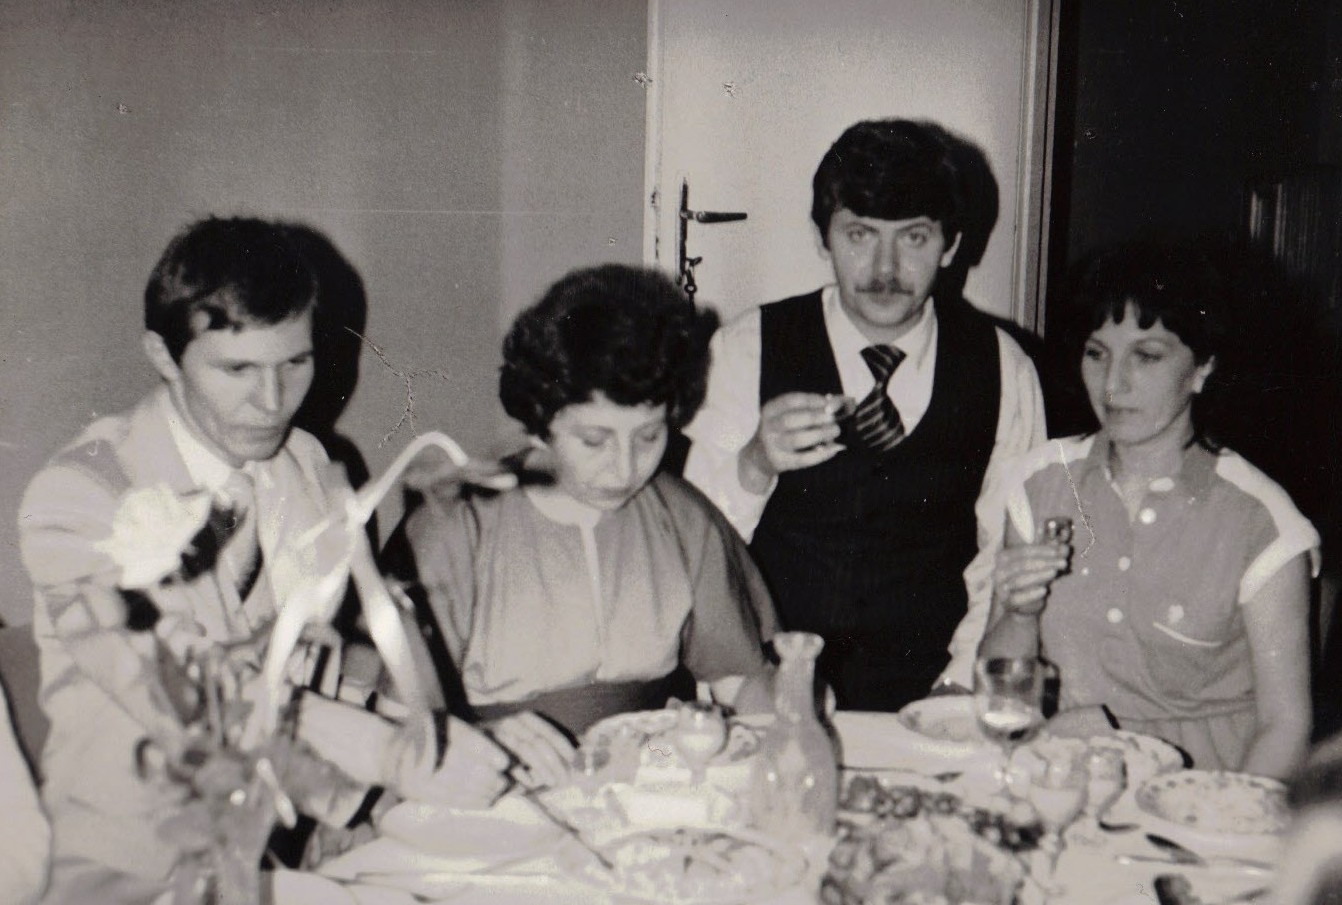
\includegraphics[width=0.7\textwidth]{zdjecia/krzysztof_karon_jarek_karon_z_zona.jpg}
\caption[Krzysztof, Jarosław i Mariola Karoniowie]{Na zdjęciu od lewej: Krzysztof Karoń, jego kuzynka Jola Czyż, brat Jarosław z żoną Mariolą}
\label{rys:krzysztof_karon_jarek_karon_z_zona.jpg}
\end{center}
\end{figure}

W 11 lat po Jarku Krzysiu Karoń znalazł tę, z którą postanowił założyć rodzinę i być jej wiernym do końca, co przyrzekł w kościele w Sędziszowie dnia 9 VI 1990 r. Wybranką była Maria Herej ur. 10 II 1967~r. w Jędrzejowie z ojca Józefa i matki Krystyny z domu Madyś. Ma z nią trójkę wspaniałych dzieci: syna Jędrzeja ur. 7 II 1991 r., córkę Magdalenę ur. 8 IX 1992 r. oraz córkę Aleksandrę ur. 16 I 1994 r., wszystkie urodzone w Kędzierzynie Koźlu.


%TODO
{\color{red}
*** Tu zdj. Małżeństwa Krzysztofa i Marii Herej z dziećmi.}